\documentclass[11pt, a4paper]{article}
\usepackage[T2A]{fontenc}
\usepackage[utf8]{inputenc}
\usepackage[serbianc]{babel}
\usepackage[left=1.5cm, top=0.5cm, bottom=1.5cm, right=1.5cm]{geometry}
\usepackage{graphicx}
\usepackage{fontspec}
\usepackage{enumerate}
\usepackage[export]{adjustbox}
\usepackage{textcomp}
\usepackage{amsmath}
\usepackage{gensymb}
\setmainfont{Ubuntu Light}

\begin{document}
\title{\vspace{-1cm}Python3 скрипте wiki}
\author{Технички детаљи функционисања скрипти, стандард је ЕС2}

\date{\vspace{-5ex}}
%\date{@}
\maketitle

{\large \textit {За сваку скрипту је потребно познавати геометријиске карактеристике пресека нпр, ширину, висину, тежиште затегнуте арматуре итд. Такође је потребно познавати карактеристичну чврстоћу бетона на притисак.}}\\
Такође је потребан и фајл $BetonPodaci.csv$ из које скрипте читају податке везане за марку бетона, узенгије итд, уколико га нема скрипте неће моћи да се покрену.

\begin{center}
	\begin{figure}[h]
	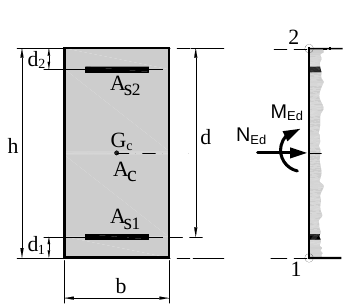
\includegraphics[width=50mm, scale=1, center]{Konvencija.png}
	\caption{Oznake i konvencija sila}
	\end{figure}
\end{center}


\begin{enumerate}

	\item {\LARGE SlozenoSavijanje.py}\\ [5mm]
	Скрипта која рачуна потребну арамтуру за комбиновано напрезање пресека услед аксијалне силе (притиска или затезања) и момента савијања.\\
	Могућности скрипте:
	\begin{itemize}
		
		\item Прорачун затегнуте арматуре за случај великог ексцентрицитета $\epsilon_{s1} \geq  2.5 \textperthousand$\\[2mm]
		Дилатација у затегнутој арматури се прорачунава аналитички при чему је радни дијаграм бетона на слици 2.
		\begin{figure}[h]
			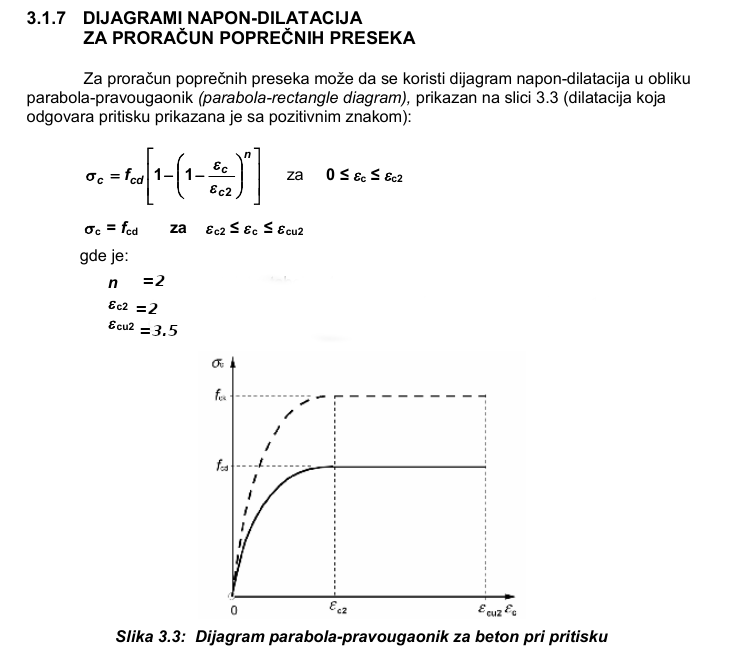
\includegraphics[width=100mm, scale=1, center]{RDB.png}
			\caption{ Радни дијаграм бетона: Парабола-Права}
		\end{figure}
		\item Двојно армирање за случај када је дилатација у затегнутој арматури $\epsilon_{s1} <  2.5 \textperthousand$
		
		\item Прорачун арматуре за случај малог ексцентрицитета\\[2mm]
	\textbf{НАПОМЕНА, ЕКСПЕРИМЕНТАЛНО:} За случај малог ексцентрицитета скрипта одређује арматуру за случај симетричног дејства момента савијања и то само у случају када је \textbf{СВА} арматура у пресеку притиснута, тј модел лома је приказан на слици 3. За сваки случај погледај дијаграме интеракције, јер је могуће да је ово погрешан приступ.
	
	\begin{figure}[h]
		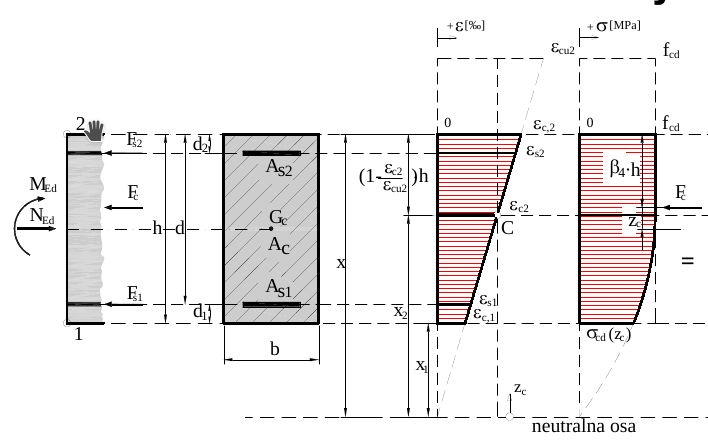
\includegraphics[width = 120mm, scale = 1, center]{MaliEks.png}
		\caption{ Модел лома за који скрипта ради мали ексцентрицитет}
	\end{figure}
За случајеве када постоји затегнута арматура услед малог ексцентрицитета скрипта ће деловати као да је "забаговала", али само покушава да пронађе равнотежу задовољавајуће тачности а не успева, зауставиће се када прође све итерације по $\epsilon_{c2} $ и избациће да је равнотежа успостављена са великом грешком. У случају обе притиснуте арматуре скрипта брзо проналази равнотежу, итерацијама по $\epsilon_{c2}$ па потом по $A_{s1}$ и коначно по $A_{s2}$ , при чему претходно наведене вредности се крећу у следећим интервалима:

\begin{align*}
	\epsilon_{c2} \in (2, 3.5)  \quad [\textperthousand]\\
	 A_{s1} \in (0, 0.04bh)  \quad [cm^2]\\
	 A_{s2} \in (0, 0.04bh)  \quad [cm^2]\\
\end{align*}

 Случајеви када скрипта користи функцију малог ексцентрицитета:
 		\begin{itemize}
 			\item Скрипта врши прорачун према двојном армирању и површина притиснуте арматуре је већа од површине затегнуте арматуре тј $A_{s2} > A_{s1}$
 			
 			\item  Напон на затегнутој ивици је већи од нуле, тј када је прва ивица притиснута: $\sigma_1 >  0$
 			
 			\item Потребна површина арматуре услед комбинованог напрезања је мања од нуле, тј $A_{s1} < 0$ за $N_{Ed} > 0; M_{Ed} \neq 0$
 			
 			\item Грешка равнотоже сила за случај малог ексцентрицитета за коју скрипта избацује резултат:
 				\begin{flalign*}
 				\Delta N &= F_{s1} + F_{s2} + F_{c} - N_{Ed} < 5 \quad [kN] \\
 				\Delta M &= F_c(d - \beta_4h) + F_{s2}(d - d_2)- M_{Ed} - N_{Ed}(h/2 - d_1) < 5 \quad [kNm]
 				\end{flalign*}
 		\end{itemize}

		\item Контрола минималног и максималног процента армирања за случај великог ексцентрицитета, при чему је:
		\begin{align*}
			A_{s,min} &= max \left\{\begin{array}{l}
				0.26\frac{f_{ctm}}{f_{yk}}b_{t}d \quad [cm^2] \\[4mm]
				0.0013b_{t}d	 \quad [cm^2]		
			\end{array} \right.\\
			A_{s,max} &= 0.473bd\frac{f_{cd}}{f_{yd}} \quad [cm^2]
		\end{align*}

\item Прорачун потребне арматуре за случај центричног притиска и  (екс)центричног затезања, за случај центричног притиска површина арматуре је:\\

\begin{align*}
As[cm^2] &= max \left\{\begin{array}{l}
0.15 \frac{N_{Ed}}{f_{yd}} \\
0.003A_c \\
4 \phi 12 = 4.52 \quad [cm^2]
\end{array} \right.\\
A_c &= bh
\end{align*}

%As = max \left\{\begin{array}{l}
%	0.15 \frac{N_{Ed}}{f_{yd}} \\
	%0.003A_c \\
	
\end{itemize}
	
	\item {\LARGE {SmicanjeITorzija.py}} \\[5mm]
	Скрипта која врши прорачун пресека оптерећеног на узајамно (и појединачно) дејство смицања и торзије. Прорачун се врши итеративно, за одговарајуће површине узенгија, сечност и размак. Усвојено је да је нагиб узенгија према оси носача $\alpha = 90\degree$, нагиб притиснутих бетонских дијагонала према оси носача $\theta = 45\degree$. Потребно је унети и површину подужне арматуре од савијања $A_{s1}$.\\[4mm]
	Могућности скрипте:
	\begin{itemize}
		\item Функција смицања:
		\begin{itemize}
		
		
		\item Прорачун потребне сечности, размака и површине узенгија 
		\item Прорачун минималног процента арматуре услед смицања $V_{Ed} < V_{Rdc}$, где је:
			\begin{align*}
				V_{Rdc} =	 max \left\{\begin{array}{l}
				0.12k(100\rho_lf_{ck})^{\frac{1}{3}}b_{w}d \quad [kN]\\
				0.035^{\frac{3}{2}}f_{ck}^{\frac{1}{2}}b_{w}d  \quad [kN]
				\end{array} \right.
			\end{align*}
			Где су:
			
			\begin{align*}
				k = 1 + \sqrt{\frac{200}{d}}, \quad k_{max} = 2, \quad d - mm\\
				\rho_l = \frac{A_{sl}}{b_wd}, \quad \rho_{l,max} = 2 \%
			\end{align*}
			
			Сечност је у овом случају $m = 2$, $\phi = 8 [mm]$ и минимални размак арматуре је:
			
			\begin{align*}
			s_{min} &= \frac{mA_{s, \phi 8}^{(1)}}{\rho_{min}b} \\
			\rho_{w, min} &= 0.08\frac{\sqrt{f_{ck}}}{f_{yk}}
			\end{align*}
			
		\item Прорачун максималног подужног растојања у зависности од интензитета траснверзалне силе:\\
		
			\begin{tabular}{|c|c|c|c|} \hline
				 &Прорачунска вредност силе смицања $V_{Ed}$ & $\leq C50/60$ & $\geq C50/60$\\ \hline
				 1 & $0.3V_{Rd,max}$ & $0.75d \leq 300mm$ & $0.75d \leq 200mm $\\ \hline
				2 & $0.3V_{Rd,max} \leq V_{Ed} \leq  0.6V_{Rd,max}$& $0.55d \leq 300mm$ & $0.55d \leq 200mm$\\ \hline
				3 &$V_{Ed} \geq 0.6V_{Rd,max} $ & $0.3d \leq 200mm$  & $0.3d \leq 200mm$\\ \hline
			\end{tabular}\\[2mm]
					
		\item Прорачун максималног попречног растојања узенгија у зависности од интензитета трансверзалне силе:\\
		
			\begin{tabular}{|c|c|c|c|} \hline
				 &Прорачунска вредност силе смицања $V_{Ed}$ & $\leq C50/60$ & $\geq C50/60$\\ \hline
				 1 & $0.3V_{Rd,max}$ & $0.75d \leq 600mm$ & $0.75d \leq 400mm $\\ \hline
				2 & $0.3V_{Rd,max} \leq V_{Ed} \leq  0.6V_{Rd,max}$& $0.75d \leq 600mm$ & $0.75d \leq 400mm$\\ \hline
				3 &$V_{Ed} \geq 0.6V_{Rd,max} $ & $0.3d \leq 300mm$  & $0.3d \leq 300mm$\\ \hline
			\end{tabular}\\[2mm]
		
		\item Контрола максималне притиснуте бетонске дијагонале, највећи проценат армирања је за сечност $m = 4$, uzengiju $\phi = 12 [mm]$,  rastojanje $s = 7.5 [cm]$, а највећа сила у притиснутој дијагонали је:
		\begin{align*}
		V_{Rd, max} &= 0.9\nu_1 bdf_{cd}\\
		\nu_1 &=  max \left\{\begin{array}{l}
		0.5\\
		0.9 - \frac{fck}{200} \quad
			\end{array}\right.
		\end{align*}
		
		\end{itemize}
		
		\item Функција торзије:
				
		\begin{itemize}
		
		\item Функција рачуна геометријиске податке по следећим обрасцима:
		 	
		 		\begin{align*}
				t_{ef} &=	 max \left\{\begin{array}{l}
					\frac{bh}{2(b+h)}\\[2mm]
					2d_1
				\end{array} \right.\\[2mm]
				b_k &= h - t_{ef}\\
				h_k &= b - t_{ef}\\
				A_k &= b_kh_k\\
				u_k&= 2*(b_k + h_k)\\
				T_{Rd,c} &= 2A_kt_{ef}f_{ctd} 
			\end{align*}
		
		\end{itemize}
		\item Функција смицања и торзије:
		\begin{itemize}
			\item НАПОМЕНА: Да бих учинио скрипту *паметнијом*, у смислу да ако корисник зада нпр. $V_{Ed} = 300  [kN], \quad T_{Ed} = 1  [kNm]$, увео сам услове да прво провери суму:
		
			$$\frac{V_{Ed}}{V_{Rd,c}} + \frac{T_{Ed}}{T_{Rd,c}} \leq 1$$\\
			Уколико услов није испуњен проверавају се и следећи услови:
			
		\begin{align}
			\frac{V_{Ed}}{V_{Rd,c}} \leq 0.05\\
			\frac{T_{Ed}}{T_{Rd,c}} \leq 0.05
	\end{align}
	Уколико је један од услова испуњен позива се функција за други начин напрезања. На пример ако је испуњен услов $(2)$ скрипта сматра да нема торзије и позива функцију смицања, важи и обрнут случај.\\
	Наравно ту је и услов лома бетонских дијагонала:
		
		\begin{align*}
			\frac{V_{Ed}}{V_{Rd,max}} + \frac{T_{Ed}}{T_{Rd,max}} \leq 1
		\end{align*}

Уколико је услов испуњен скрипта ради итеративан прорачун површине узенгија, сечности и размака. Уколико није скрипта избацује поруку прекорачења услова и штампа $V_{Rd,max}$ и $T_{Rd, max}$.	
	
					 
		\end{itemize}
		
	\end{itemize}	
	
\item {\Large{MomentNosivosti.py}}\\[5mm]
Скрипта која врши прорачун носивости правоугаоних пресека оптерећених сложеним савијањем, пресеци могу бити са и без притиснуте арматуре.\\[2mm]
Разматрају се два случаја, када постоји и када не постоји притиснута арматура која се узима у обзир.
Уколико не постоји прорачунска притиснута арматура (случај $A_{s2}=0$), и уколико је услов $\epsilon_{s1} \geq 2.5 \perthousand$ прорачун се врши аналитички преко коефицијента $\xi$ и исписује се носивост, уколико је $\epsilon_{s1} < 2.5 \perthousand$ момент носивости се рачуна итеративно уз задовољење равнотеже аксијалних сила:

\begin{align*}
	\Delta N &= F_{c} - F_{s1} - N_{Ed}\\
	\Delta N &\leq 0.5 \quad [kN]\\[2mm]
	\end{align*}

Где су:	
	
$Fc- \text{Сила у притиснутом бетону}$\\
$F_{s1}-\text{Сила у затегнутој арматури}$\\
$\Delta N -\text{Грешка равнотеже сила}$

За случај постојања прорачунске притиснуте арматуре ($A_{s2} > 0$), прорачун се врши итеративно уз задовољење претходне равнотеже сила уз исту тачност, само што у равнотежи фигурише и $F_{s2}$.

\item {\Large{Naponi.py}}\\[5mm]
Скрипта која врши прорачун и контролу напона са и без притиснуте арматуре, са случај момента за пресек са прслином.\\
НАПОМЕНА: Дејствујући момент $M_{ed}=M$ се уноси за SLS комбинацију дејства, било за карактеристичну или квази-сталну комбинацију, приликом штампања резултата ће скрипа показати која контрола је прекорачена, корисник треба да увиди за коју комбинацију врши контролу и да изабере од резултата шта му је потребно.\\
Коефицијент $\xi$ се рачуна по следећем обрасцу.

\begin{align*}
	\xi=\alpha\left(\rho_{1}+\rho_{2}\right)(-1+\sqrt{1+\frac{2\left(\rho_{1}+\rho_{2} \frac{d_{2}}{d}\right)}{\alpha\left(\rho_{1}+\rho_{2}\right)^{2}}})
\end{align*}
Напон у бетону:
\begin{align*}
	\sigma_{c}=\frac{M}{b d^{2}} \frac{1}{\frac{\xi}{2}\left(1-\frac{\xi}{3}\right)+\alpha p_{2}\left(1-\frac{d_{2}}{\xi d}\right)\left(1-\frac{d_{2}}{d}\right)}
\end{align*}
Напон у притиснутој арматури:
\begin{align*}
	\sigma_{s 2}=\alpha \sigma_{c} \frac{\xi-\frac{d_{2}}{d}}{\xi}
\end{align*}
Напон у затегнутој арматури:
\begin{align*}
	\sigma_{s 1}=\alpha \sigma_{c} \frac{1-\xi}{\xi}
\end{align*}

Скрипта ће исписати уколико напони у бетону или арматури пролазе следеће контроле.
Квази-стална комбинација: 
\begin{align*}
	\sigma_c &\leq 0.45f_{ck}\\
	\sigma_{s1} &\leq 0.8f{yk}
\end{align*}
Карактеристична комбинација:
\begin{align*}
	\sigma_c &\leq 0.6f_{ck}\\
	\sigma_{s1} &\leq 0.8f{yk}
\end{align*}

\item {\Large{Prsline.py}}\\	[5mm]

Скрипта која врши прорачун и контролу ширине прслина за пресеке без преднапрезања напрегнуте на савијање са ребрастом арматуром. Потребно је претходно познавати напон у арматури.\\
Могућности скрипте:

\begin{itemize}
	
	\item Могућност прорачуна за краткотрајно и дуготрајно оптерећење.
	
	\item Исписивање и максималног размака прслина  $s_{r,max}$
	
Препоручене карактеристичне ширине прслина $w_k$  по ЕС2 [mm]:\\

\begin{tabular}{|p{6cm}|p{6cm}|}
\hline
 Класа изложености & Армирано бетонски и претходно напрегнути елементи са кабловима без приањања са бетоном\\
& Квази-стална комбинација оптерећења\\
\hline
$X0, XC1$ & $0.4$\\ 
\hline
$XC2, XC3, XC4$ & 0.3\\ 
\hline
$XD1, XD2, XD3, XS1, XS2, XS3$ & 0.3\\
\hline 
\end{tabular}\\[2mm]
Прорачун се врши по следећим обрасцима:
\begin{align*}
	w_k &= s_{r,max}(\epsilon_{sm} - \epsilon_{cm})\\
	\varepsilon_{\mathrm{sm}}-\varepsilon_{\mathrm{cm}}&=\frac{\sigma_{\mathrm{s}}-k_{\mathrm{t}} \frac{f_{\mathrm{ct}, \text { eff }}}{\rho_{\mathrm{p}, \text { eff }}}\left(1+\alpha \rho_{\mathrm{p}, \mathrm{eff}}\right)}{E_{\mathrm{s}}} \geq 0.6 \frac{\sigma_{\mathrm{s}}}{E_{\mathrm{s}}}\\
	\rho_{p.eff} &= \frac{A_{s}}{A_{c.eff}}\\
	A_{c,eff} &= bh_{ceff}\\
	h_{c,eff} &= min \left\{\begin{array}{l}
	2.5(h - d)\\[2mm]
	\frac{h-x}{3}\\[2mm]
	h/2\\
	\end{array}
	\right.	
\end{align*}
Максимално растојање прслина:\\
\begin{align*}
	s_{r,max} &= k_3c + k_1k_2k_4\frac{\emptyset}{\rho_{p.eff}}\\
	k_3 &= 3.4\\
	k_4 &= 0.425\\
	\emptyset = \emptyset_{eq} &= \frac{n_1\emptyset_1^2+n_2\emptyset_2^2}{n_1\emptyset_1 + n_2\emptyset_2}\\
	k_1 &= 0.8\\
	k_2 &= 0.5
\end{align*}
\end{itemize}

\item {\Large {MomentKrivina.py}}\\[5mm]
Скрипта која штампа дијаграм момент-кривина за минималу, максималну, и површину арматуре унету од стране корисника. Након уноса аутоматски се приказује дијаграм са 3 криве (или две у зависности од прорачуна) и чува се фајл под називом $Stampa.png$. Прво одређује момент-кривину при појави прслине а потом итеративно мења $\epsilon_c$  за случај течења арматуре $\epsilon_{s1} = 2.175 \perthousand$, уколико се не постигне равнотежа ни за једно $\epsilon_c$ усваја се да је $\epsilon_c = 3.5 \perthousand$ и итерира се по $\epsilon_{s1}$. Дијаграми се цртају спајањем карактеристичних тачака: Приликом штампања дијаграма корисник има могућност да сачува одштампани дијаграм.\\
\begin{itemize}

	\item Прва тачка $(M, \kappa)$ при којој се јавља прва прслина
	
	\item Друга тачка $(M, \kappa)$ при дилатацији течења арматуре $\epsilon_{s1} = 2.175 \perthousand$
	
	\item Трећа тачка $(M, \kappa)$ је при лому бетона, $\epsilon_c = 3.5 \perthousand$
\end{itemize}
 Приликом штампања дијаграма корисник има могућност да сачува одштампани дијаграм.\\
Могућности скрипте:
\begin{itemize}
	\item Исписивање у терминалу (PowerShell-u) карактеристичне тачке дијаграма, тј њихове тачне вредности момента и кривине
	
	\item Скрипта (засад) НЕ ради пресеке са утегнутим бетоном, максимална дилатација у бетону је $3.5 \perthousand$!
	
	\item Скрипта ради само са затегнутом арматуром
\end{itemize}
Равнотежа унутрашњих сила зависи само од сила у бетону и затегнутој арматури, скрипта избацује решење са грешком равнотеже сила: $\Delta N \leq 0.5$ $[kN]$


\item {\Large{UtezanjeStuba.py}}\\[5mm]
Скрипта која врши контролу нормализоване силе у стубу и даје потребне пречнике узенгија и њихов размак за дату геометрију пресека за елементе којима је потребно да испуне средњу класу дуктилности DCM.\\
НАПОМЕНА: Потребно је имати потпуно дефинисан пресек (размак придржаних шипки, број придржаних шипки, ширину утезања, обим шипки за утезање итд) као и динамичке податке (период осциловања конструкције итд). Скрипта итеративно проверава за сваки пречник узенгија  $\emptyset8, \emptyset10, \emptyset12$, респективно уз минимални размак од $7.5$ $[cm]$ и максимални размак од $20$ $[cm]$. Итерира се прво за $\emptyset8$ на $20$ $[cm]$ до $\emptyset12$ на $7.5$, и када скрипта наиђе на први размак који задовољава утезање за одређени пречник шипке прећи ће на следећи (већи) пречник и поновити итерирање од највећег размака, са овим корисник има у виду варијантна решења. Уколико не испуни услове утезања за $\emptyset12$ на $7.5$ $[cm]$ избациће коментар да је недовољно утезање пресека.
\end{enumerate}

\LARGE{Ово је кратак опис начина рада скрипти, попуњаваћу овај wiki са времена на време, грешке су могуће и у wiki-ју и у раду скрипти, резултате посматрај са одрећеном дозом скептицизма.}\\

\Large{Сав feedback је добродошао на $nikola@lakic.one$}

\end{document}